
%(BEGIN_QUESTION)
% Copyright 2011, Tony R. Kuphaldt, released under the Creative Commons Attribution License (v 1.0)
% This means you may do almost anything with this work of mine, so long as you give me proper credit

Explain how all valve positioners essentially act as {\it cascade} control systems in a loop, and why valve positioners generally improve control quality as a result.

\vskip 10pt

Furthermore, examine this block diagram of an electronic (``smart'') valve positioner and comment on its own internal ``control strategy'' for achieving optimum positioning:

$$\includegraphics[width=15.5cm]{i01691x01.eps}$$

\vskip 20pt \vbox{\hrule \hbox{\strut \vrule{} {\bf Suggestions for Socratic discussion} \vrule} \hrule}

\begin{itemize}
\item{} Comment on the ``+'' and ``$-$'' symbols shown in this diagram.  Based on these symbols, determine the control action (direct or reverse) for each of the controllers.
\item{} Certainly, modern ``smart'' valve positioners promise superior control valve performance than mechanical valve positioners did.  Can you think of any potential {\it disadvantages} of a smart valve positioner, especially after examining the block diagram in detail?
\item{} For those who have studied control valve positioners, how exactly does a ``smart'' positioner sense the valve stem's position?
\item{} For those who have studied control valve positioners, identify some of the special features offered by a ``smart'' positioner.
\item{} Predict the effect(s) of the nozzle plugging inside the positioner's relay.
\item{} Predict the effect(s) of the travel sensor failing with a 0\% (fully-closed) signal.
\item{} Predict the effect(s) of the pressure sensor failing with a 100\% (full-pressure) signal.
\end{itemize}

\underbar{file i01691}
%(END_QUESTION)





%(BEGIN_ANSWER)

Electronic valve positioners act as controllers of a sort by sensing stem position (PV), comparing that PV against the command value coming from the loop controller (the positioner's SP), and finally generating its own pneumatic output signal to drive the actuator and move the valve to where it should be.

\vskip 10pt

A potential problem with electronic positioners is the potential to mis-tune its internal control(lers), resulting in oscillations if the internal control is too aggressive and sluggishness if the internal control is not aggressive enough.  

%(END_ANSWER)





%(BEGIN_NOTES)

A valve positioner is essentially nothing more than a proportional-only position controller.  The signal a positioner receives from a controller is a setpoint for the valve stem position.  The positioner then takes action to drive the actuator as much or as little as necessary to ensure the stem position is equal with the ``setpoint'' given by the external controller.

Because of this secondary control action, phenomena such as dynamic forces on the valve plug, packing stiction, and other factors will have less impact on the overall control quality than if there was no positioner in use at all.  In effect, positioners ``decouple'' such effects from the master control system.

\vskip 10pt

Some engineering texts state that valve positioners often degrade the performance of inherently fast processes such as liquid flow by introducing another time lag into the loop.  However, pneumatically-actuated valves tend to be quite slow without the high volumetric flow rate of compressed air afforded by a positioner, and so positioners actually speed up valve action considerably when compared against pneumatic valves powered by I/P transducers alone.

%INDEX% Control, strategies: cascade

%(END_NOTES)


